\documentclass{article}
\usepackage{graphicx} % Required for inserting images
\usepackage{amsmath}

\title{DISCO Summary}
\author{Hang Su}
\date{June 2023}

\begin{document}

\maketitle

\section{Solutions to the Disco Primer}
Fluids are defined by spacetime dependent quantites: mass density $\rho$, velocity $v$, and pressure $P$.
In case of the accretion disks of a black hole, we have $5$ real variables: $\rho$, $P$, and $3$
components of $v$. We also have $5$ equations for the $5$ variables along with sonservation laws: 
\begin{enumerate}
    \item Conservation of particle number
    \item Conservation of momentum
    \item Conservation of energy.
\end{enumerate}

These conservation laws give us the equations needed to solve: the Continuity Equation, Euler Equations,
and the Energy Equation.
\begin{eqnarray}
    && \partial_t \rho + \nabla (\cdot \rho v) = 0 \nonumber \\
    && \partial_t (\rho v) + \nabla \cdot (\rho vv + P) =  \rho g \nonumber \\
    && \partial _t (\frac{1}{2} \rho v^2 + e) + \nabla \cdot \left[\left(\frac{1}{2
    } \rho v^2 + e + P \right) v \right] = \rho v \cdot g - \dot q
\end{eqnarray}

The goal for DISCO code is to solve these equations for a hydrodynamic system. Below I have documented
the process of which I preliminarily solve these equations using analytical methods to give rise to 
a simple disk model. 

\subsection{Steady and axissymmetric}

We assume the disk model to be long-lived and axisymmetric. That is, the disk will look the same
from any angle at any moment of time. Thus, we set derivatives of time and angle $\phi$ in cylindrical coordinates
to $0$. Here we will have four ordinary differential equations:

\begin{eqnarray}
    && \textit{Continuity: } \frac{1}{r} \partial_r (r \Sigma V_r) = 0 \nonumber \\
    && \textit{Radial Momentum: } \frac{1}{r} \partial_r \left(r \Sigma 
    V_r^2 + r \Pi - 2r \Sigma \nu \left(\frac{2}{3} \partial_r V_r - 
    \frac{1}{3} \partial_\phi \Omega\right)\right) = 0 \nonumber \\
    && \textit{Angular Momentum: } \frac{1}{r} \partial_r \left(r^3 
    \Sigma V_r \Omega - 2 r \Sigma \nu \left(\frac{1}{2} r^2 \partial_r \Omega\right)\right)
    = 0 \nonumber \\
    && \textit{Energy: } \frac{1}{r} \partial_r \left(r \left(\frac{1}{2} \Sigma v^2
    + \Sigma \epsilon + \Pi\right) V_r - 2r\Sigma \nu(\sigma \cdot v ) r\right)
    = \Sigma v\cdot g - \dot q
\end{eqnarray}

where $\nu$ is viscosity and $\dot q$ is a cooling term, $\Omega $ is angular velocity, 
and
\begin{eqnarray}
    && v \cdot g = -\frac{GM}{r^2} \cdot v \nonumber \\
    && \Sigma = \int \rho dz.
\end{eqnarray} 

\subsection{The razor thin limit}
We are assuming that the disk is razor thin and inviscid. Here we take the approximations of
$H \simeq 0$ and $\nu = 0$. We also set the sounds speed $c_s = 0$, as well as $\Pi$ and $\epsilon$.
Here we find the solutions of  $V_r (r)$ and $\Omega (r)$.

We can do so by taking the insides of the first and third equation as constants, and solve for the other two
equations using results obtained from it. Eventually, we get one of the solutions similar to Saturn's rings: 
$V_r = 0$ and 
\begin{equation}
    \Omega = \sqrt{\frac{GM}{r^3}}.
\end{equation}

As we take the raidal velocity as $0$, we are assuming that the gas stays in a steady orbit without moving inward or
outward. This makes sense in our razor thin and axisymmetric approximation but it is unrealistic since accretion does not
occur with $V_r = 0$.

\subsection{The Accretion Rate and Torque}
We define the accretion rate $\dot M$ as the rate at which matter passes a praticular radius mobing
toward the central object: $\dot M = -2 \pi r \Sigma v_r$. From the continuity eqaution from step 1, we can derive 
\begin{equation}
    \partial_r (r\Sigma V_r) = 0
\end{equation}
and $\dot M = -2 \pi r \Sigma V_r = \textit{constant}$. This means that for a disk that is
steady and axisymmetric, the accretion rate is constant across all radii.
Later, we will use the expression of $V_r$ to solve for other quantities.
\begin{equation}
    V_r = \frac{\dot M}{-2\pi r \Sigma}
\end{equation}

Similarly, we define the torque through the disk $\dot J$ as the rate at which the central object accretes
angular momentum, which is equal to $2\pi$ times the angular momentum flux. 
From the angular momentum equation from step 1, we have
\begin{equation}
    \frac{1}{r} \partial _r (r^3 \Sigma V_r \Omega - r^3 \Sigma \nu \partial_r \Omega) = \partial_r \dot J = 0. 
\end{equation}
Using $V_r$ from above, we get 
\begin{equation}
    \dot J = \dot M r^2 \Omega + 2\pi r^3 \Sigma \nu \partial_r \Omega.
\end{equation}
Rearrange, we have an expression for $\Sigma$
\begin{equation}
    \Sigma = \frac{\dot J - \dot M r^2 \Omega}{2\pi r^3 \nu \partial_r \Omega}.
\end{equation}

\subsection{An accretion disk}

So far, we have two algebraic equations involving $\dot M$ and $\dot J$ and the radial momentum and energy equations. 
It is time to solve the final radial momentum equation assuming the disk is thin $H \ll r$ abd the radial velocity
subsonic $|v_r| < c_s$. The centripital acceleration term should balance the term with the largest other term, in this case, 
$r\Sigma \frac{GM}{r^2}$. This confirms the expression for angular velocity $\Omega = \sqrt{\frac{GM}{r^3}}$.

After simplifying, we obtain the final solution for $\Sigma$
\begin{equation}
    \Sigma = \frac{-1}{3\pi \nu} \left(\frac{\dot J}{\sqrt{GMr}} - \dot M\right),
\end{equation}

and for $V_r$ 
\begin{equation}
    V_r = -\frac{3\nu}{2r}.
\end{equation}

From here, we have obtained a series of constants and expressions that will help the DISCO code solve the hydrodynamic equations.

We define function $f$:
\begin{equation}
    f = 1 - \frac{\dot J}{ \dot M \sqrt{GMr}}.
\end{equation}

Finally, some expressions in terms of $f$:
\begin{eqnarray}
    && \Sigma = \frac{\dot M f }{ 3 \pi \nu} \nonumber \\
    && V_r = \frac{3\nu}{-2rf} \nonumber \\
    && \Omega = \sqrt{\frac{GM}{r^3}}.
\end{eqnarray}


\section{Instructions on using the DISCO code}

Now that we have analytically solved solutions of a simple disk model, it is time that we put these varaibles into the 
disco code. There are many tempates for different simulations performed in disco, but in our case we only focus on
thin accretion disk for singular or binary black holes. 

In order to run the code, we need to provide initial conditions and the instructions for the computer to run the simulations.
I have listed below some of the useful tips for this project running on disco.

The \texttt{Makefile\_opt.in} file contains the initial condition file we will use. We can specify the file name after

\begin{verbatim}
    INITIAL = {FILENAME}.
\end{verbatim}

The file we are putting into the initial section of texttt{Makefile\_opt\.in} is stored in the texttt{initial} directory. 
In this texttt{\.c} file, we can specify the disk model we are using. We can load quantities such as viscocity and adiabatic index into the file using
texttt{setICparams()} function. This is the place we can put the simple disk model we derived above into the simulation.
Specifically, these formulas are in this file:

\begin{eqnarray}
    && f = 1 - \frac{\dot J}{ \dot M \sqrt{GMr}} \nonumber \\
    && \Sigma = \frac{\dot M f }{ 3 \pi \nu} \nonumber \\
    && V_r = \frac{3\nu}{-2rf} \nonumber \\
    && \Omega = \sqrt{\frac{GM}{r^3}}.
\end{eqnarray}



If we want to have a circumbinary black hole simulation, we can add mass profiles in the texttt{planet} directory. 



In the file texttt{in\.par}, we can specify parameters such as the periods of rotation, time step, grid dimensions, hydro parameters etc.
In our practice so far, we only run a small number of checkpoints and observe the simulation through texttt{vdisco}, a visual
platform of which the checkpoints of the simulation can be vidualized. 

In vdisco, the numbers on your keyboard switches among the variables:
\begin{enumerate}
    \item [1] Surface density ($\rho$ or $\Sigma$ in derivations above)
    \item [2] Pressure $P$
    \item [3] Radial velocity $V_r$
    \item [4] Angular velocity $\Omega$
    \item [5] Vertical velocity $V_z$ ($0$ most of the times)
    \item [6] Passive scalar for visualization 
\end{enumerate}



\section{Results}

There are two key points we focused on for our results. We investigated some of the properties of eccentricities of the orbits and their effects on the accretion disks, and 
we looked at minidisks around individual black holes and their properties.

\subsection{Eccentricities}

BBHs with eccentric orbits have not been studied extensively. 
The time evolution of the orbits and minidisks is chaotic and creates 
overdensity regions that theoretical models do not predict. We have launched multiple eccentric 
runs on the Symmetry cluster with Python analysis to see if there is a stable eccentricity point, 
at which the eccentricity of the orbit stays in the same shape across a long time steps.
 However, it is worth pointing out that for all eccentricities, the cavities
 around the binary precess and eventually become eccentric.

We generated 1 checkpoint per orbits and used it to calculate many aspects of the accretion disk. 
As the orbit increases toward 1000 orbits, the surface density reaches a steady value since the gas becomes more uniform toward the bigger radii. 
Radial velocity reaches zero due to the steady state of the disk, which means gas does not move inward or outward at larger radii.
The mass accretion rate is chaotic near the center of the disk due to individual black hole's effects and the lump around the cavity, 
but it reaches a steady value at larger radii at a constant value, which means the amount of matter being accreted throughout the radial coordinates
is constant. The plot below shows the surface density, radial velocity, and mass accretion rate as a function of radius for the last 500 orbits averaged over time, where the eccentricity is 0.4.

\begin{figure}[h]
    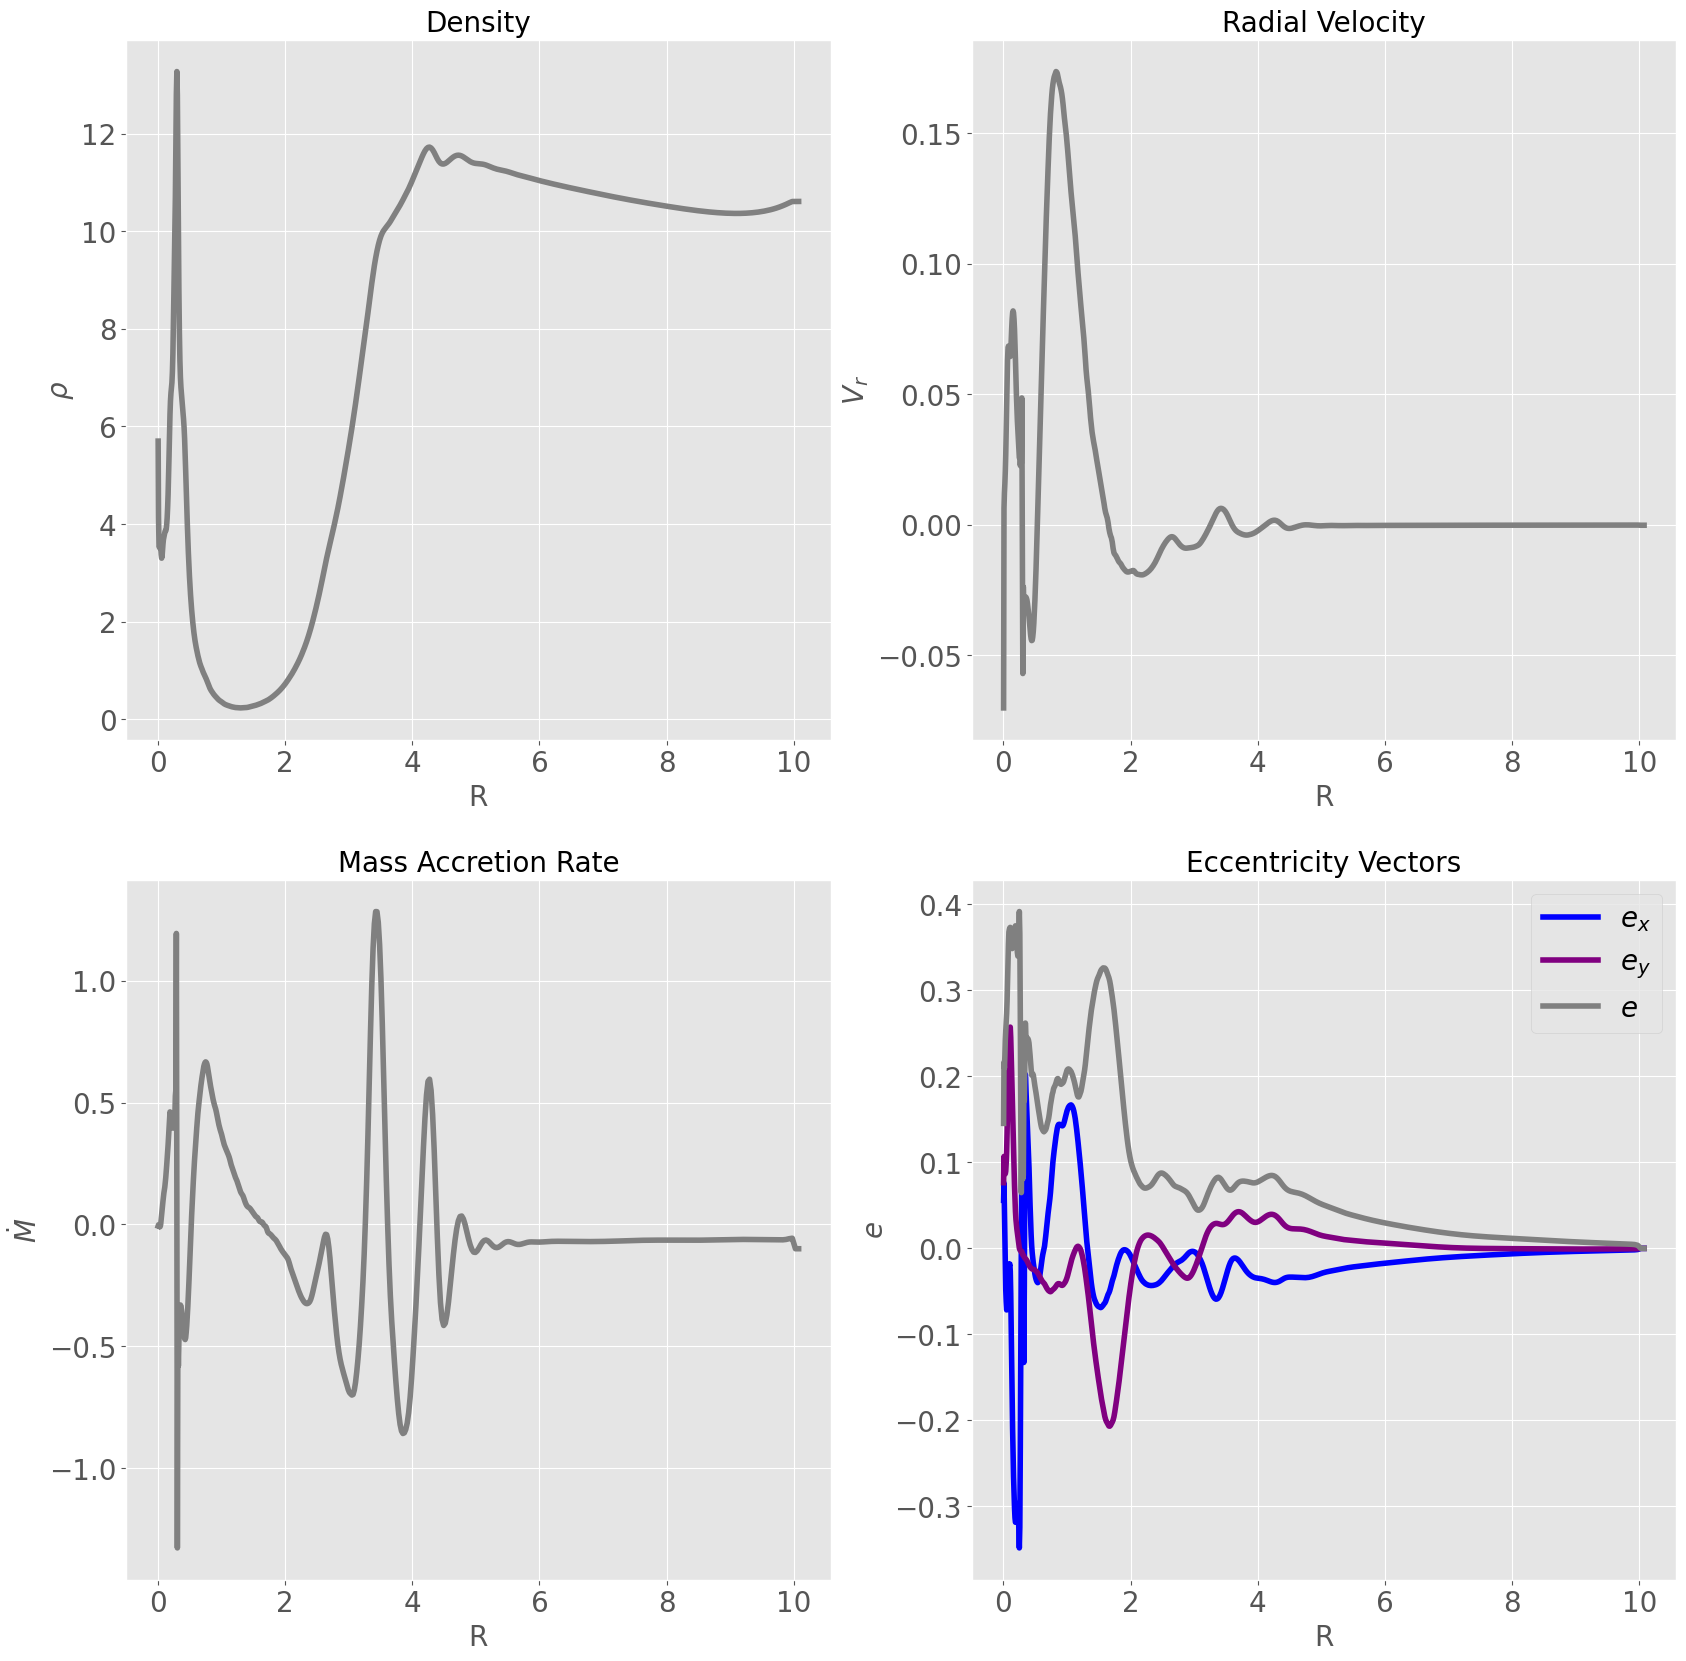
\includegraphics[width=6cm]{output.png}
    \centering
    \end{figure}

Additionally, we looked for a stable ecccentricity point for euqal mass black holes for about 1000 orbits. We found that the eccentricity is stable at 0.4, and the plot below shows the eccentricity as a function of time.
Stable eccentrity point indicates that the shape of the eccentric orbit does not change over time, and the orbit is not circular. The below shows the edot as a function of time in orbits, where the eccentricity is stable at 0.4.
For eccentricities that have positive edot, the orbit is getting more eccentric over time, and for eccentricities that have negative edot, the orbit is getting more circular over time.

\begin{figure}[h]
    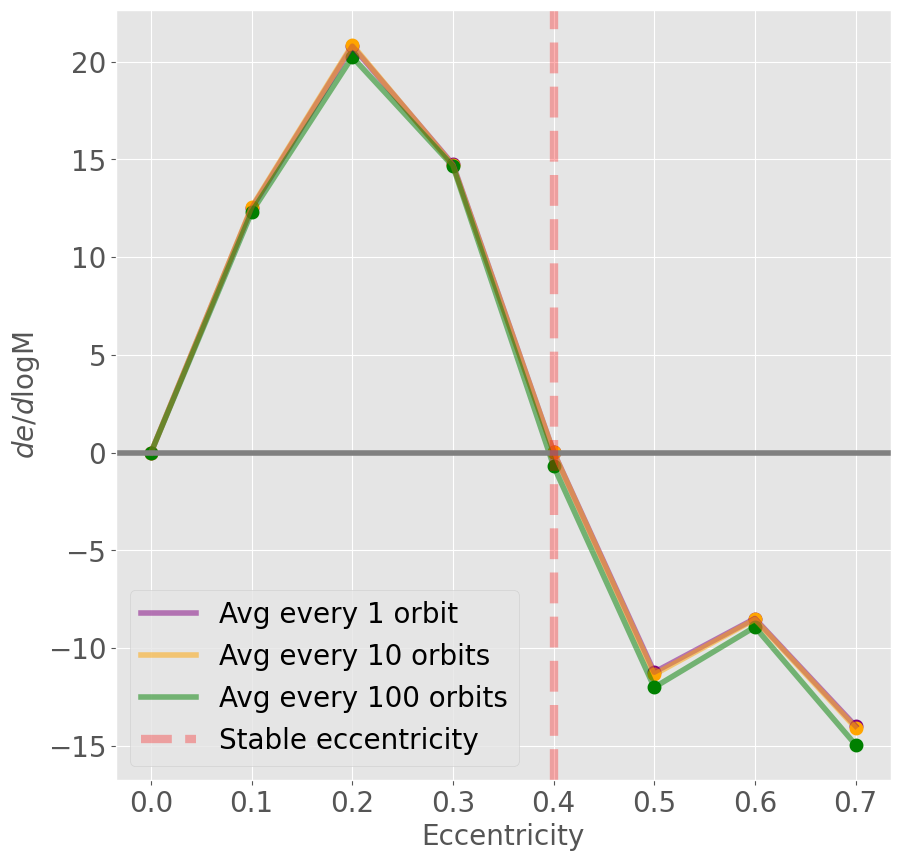
\includegraphics[width=6cm]{stable_ecc.png}
    \centering
    \end{figure}


\subsection{Minidisks}
Minidisks contain the amount of gas gravitationally bound to only one black hole in a binary system. The exact radius of a minidisk can be difficult to determine. In this work, we use the minimal mean density as the cutoff.
At small radii, the major behavior of the accretion disk is governed by minidisks around individual black holes. Below is one of the density
 plots of surface density for 0.4 eccentricity, 
 \begin{figure}[h]
    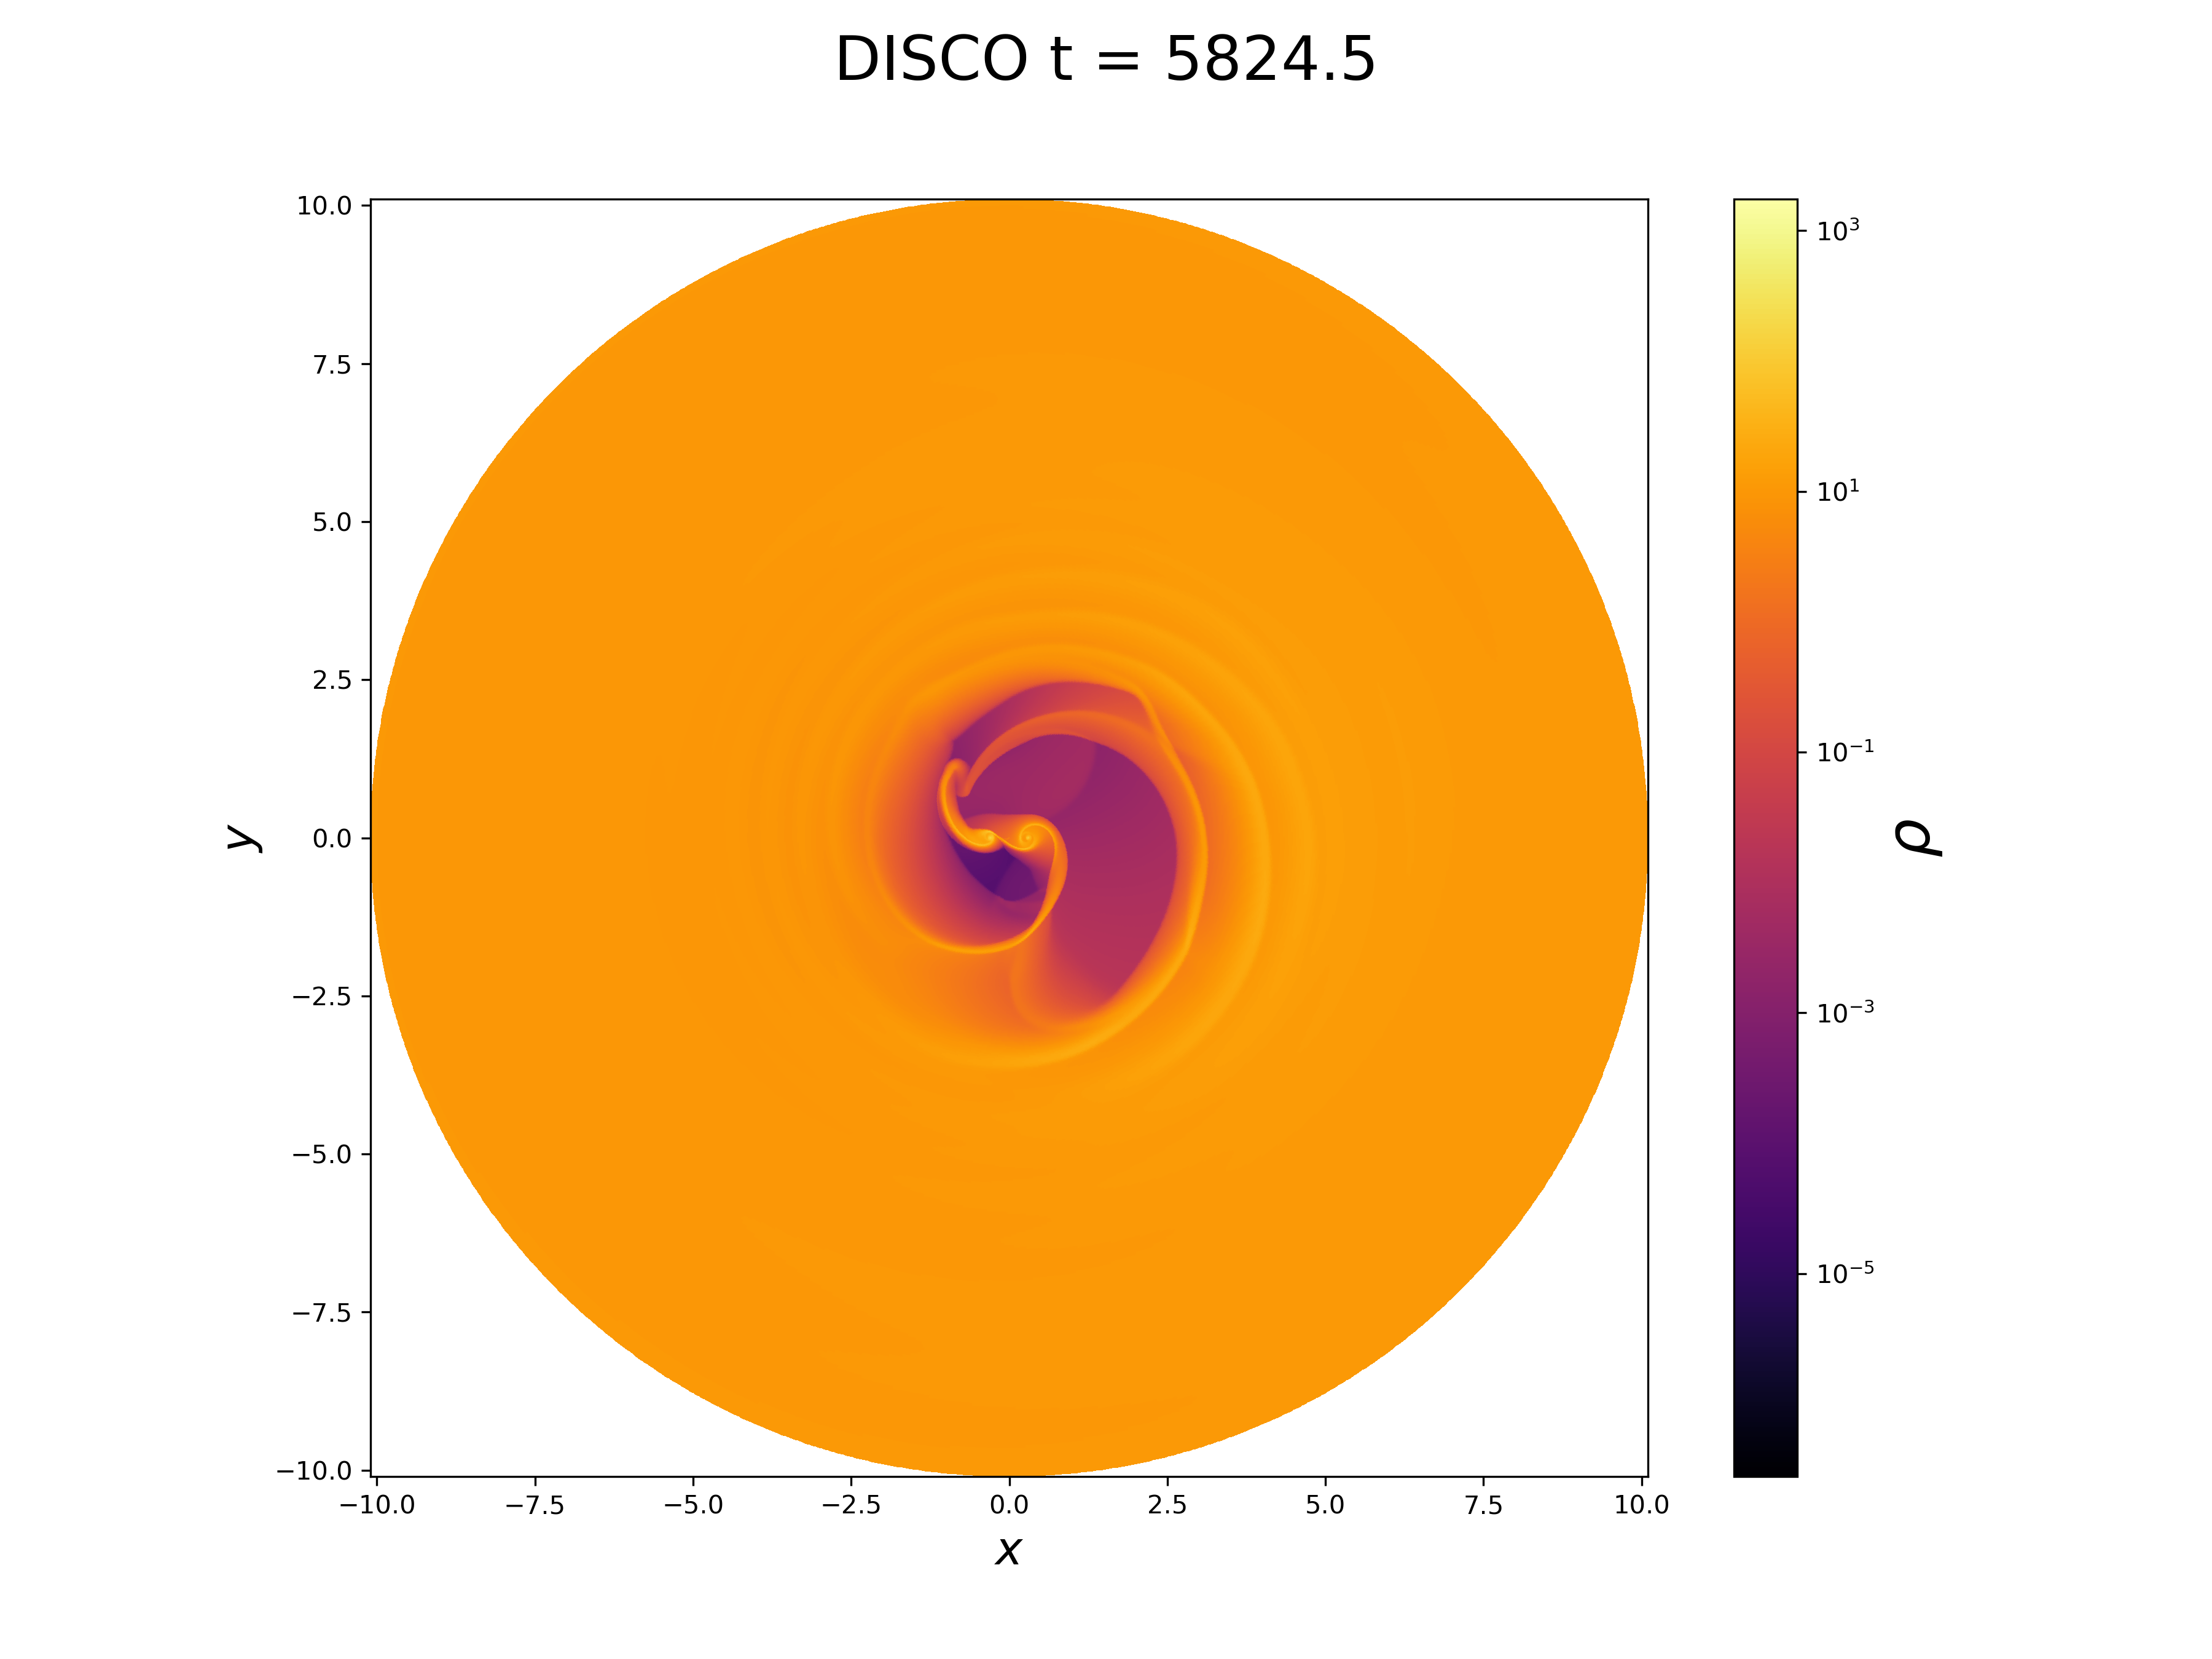
\includegraphics[width=6cm]{plot_eq_0927_log_rho.png}
    \centering
    \end{figure}
 
Plot below is the top plot zoomed in 10 times to show the minidisks.

\begin{figure}[h]
    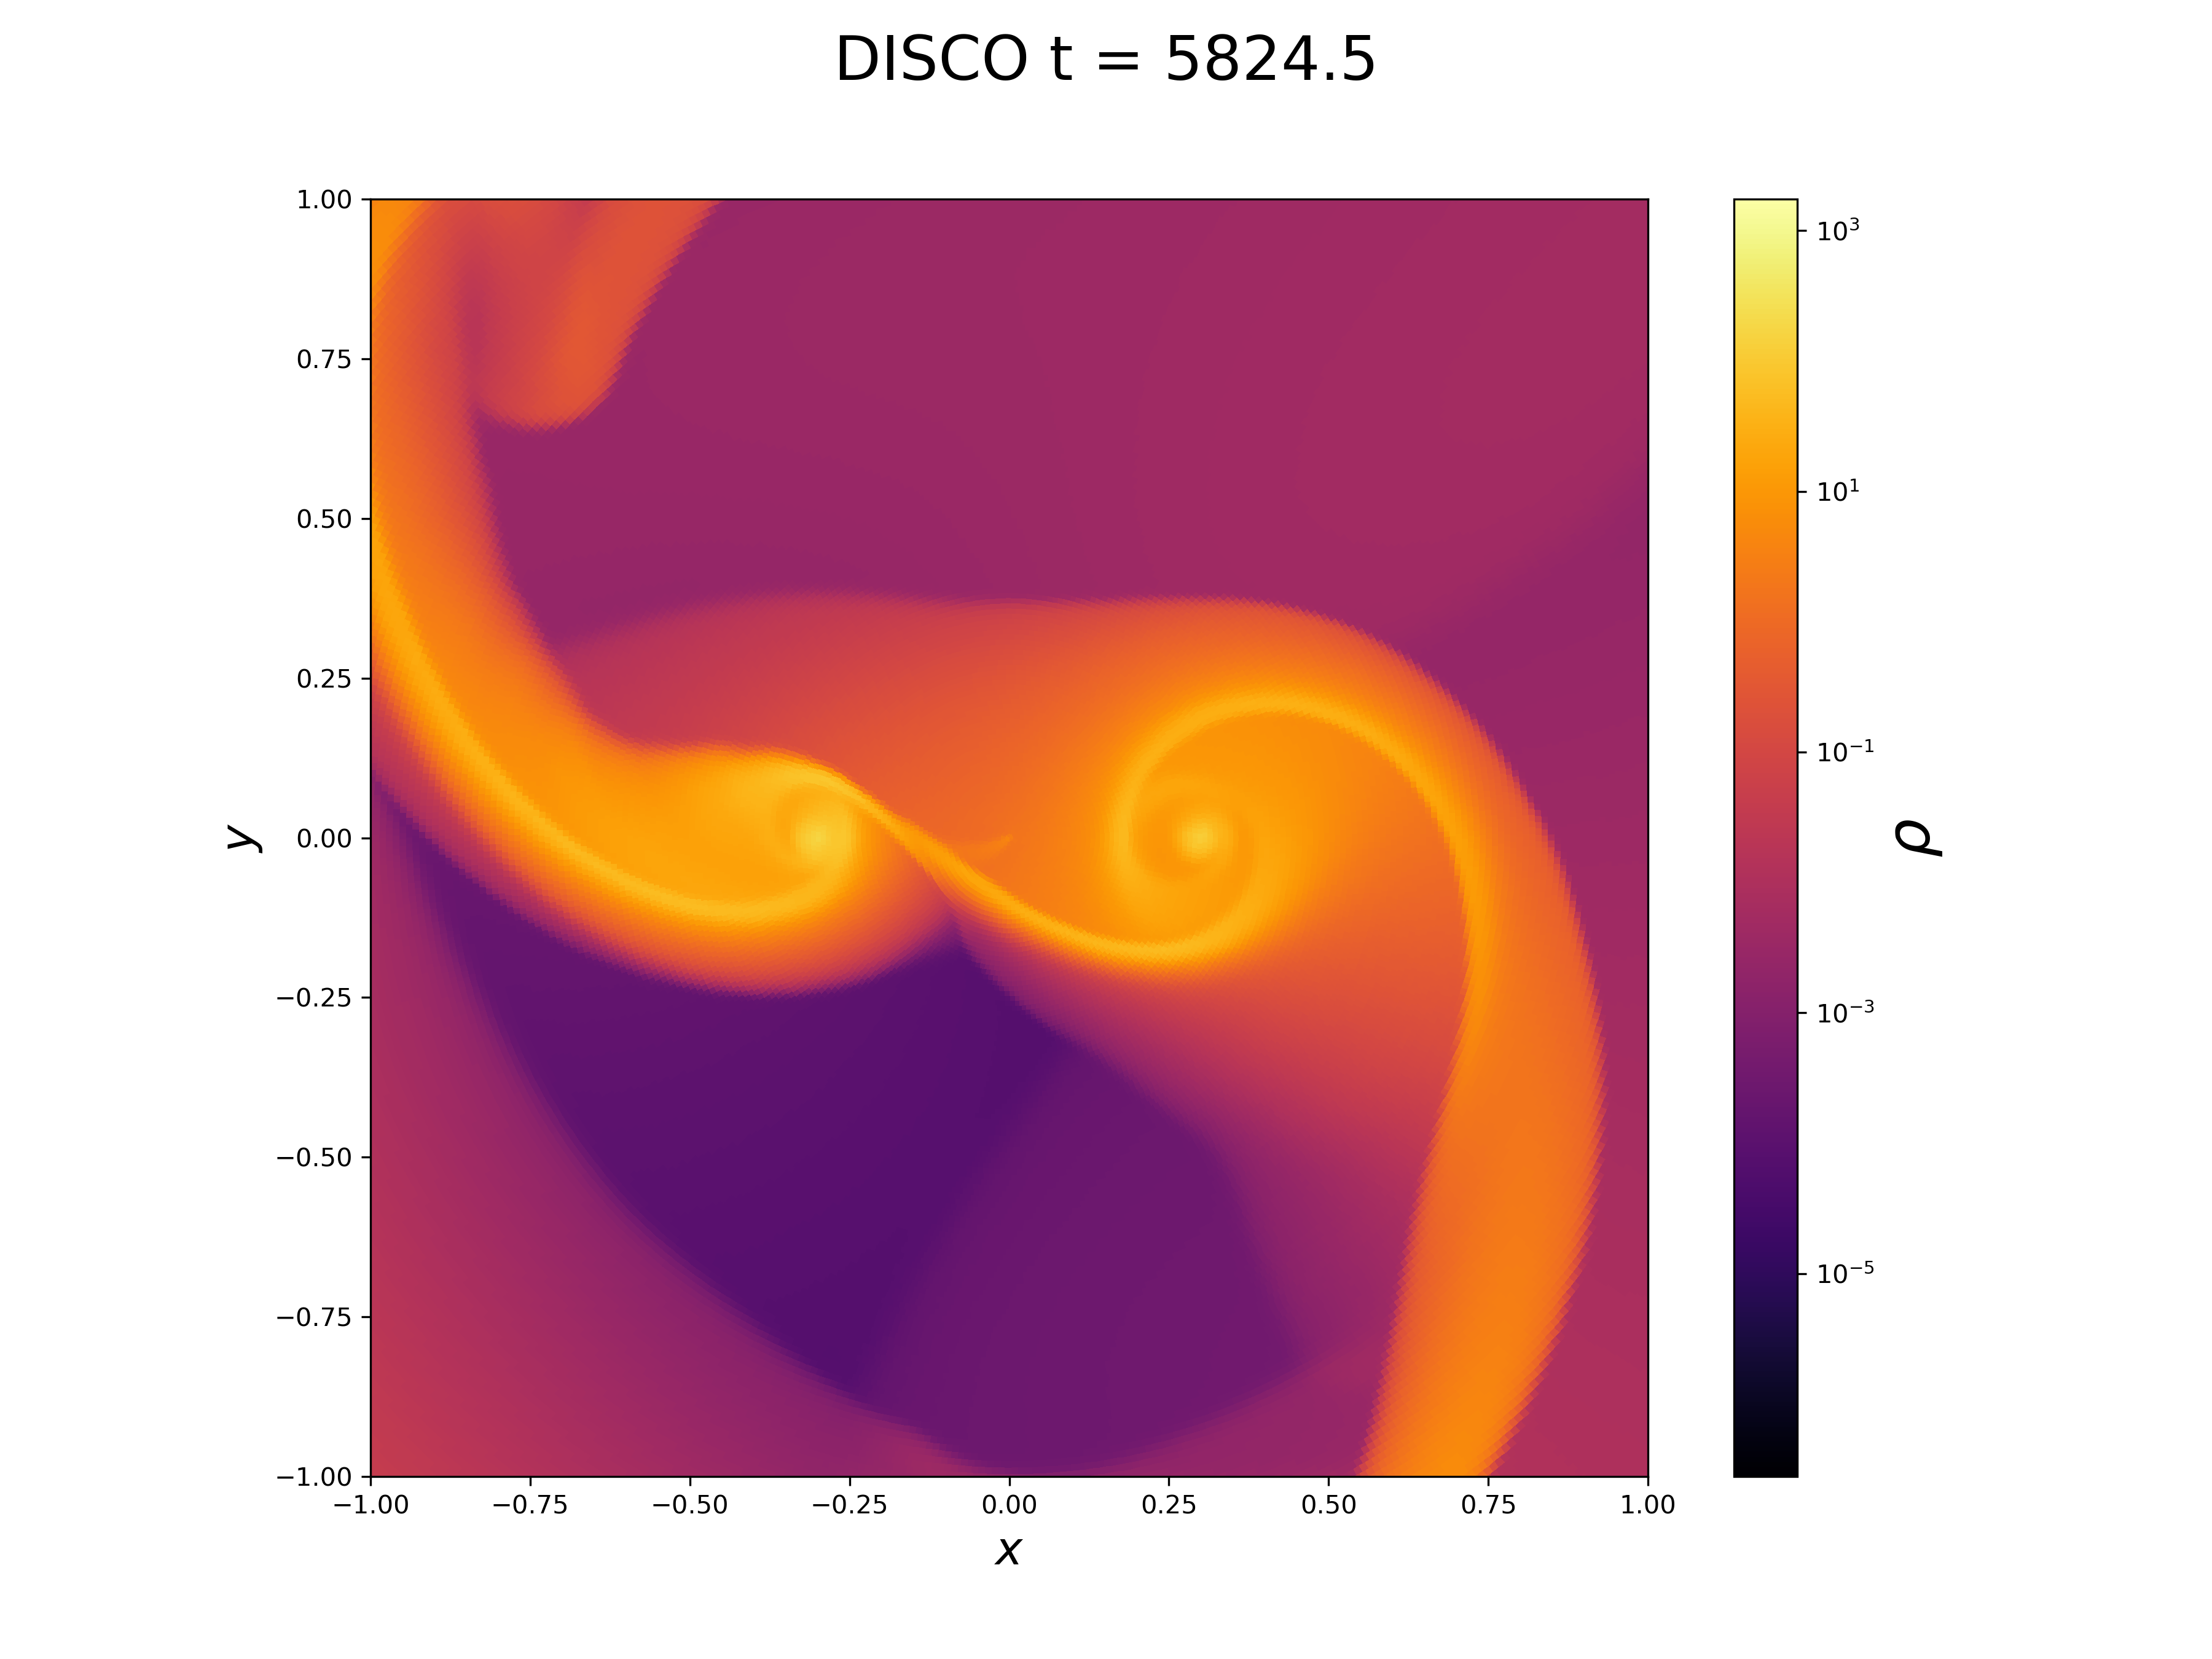
\includegraphics[width=6cm]{zoom_in.png}
    \centering
    \end{figure}

The plot below shows the total mass of one of the minidisks in different 
eccentric runs averaged every 100 orbits and then averaged into one value. 
It only plots values in the range of 400th to 500th orbits. 
The total mass at 0.2 eccentricity is smaller than other eccentricities at this time step, 
potentially due to a large time derivative of eccentricity. This indicates that we need to increase the total time for each run so that they can reach steady state before stablizing the total mass.

\begin{figure}[h]
    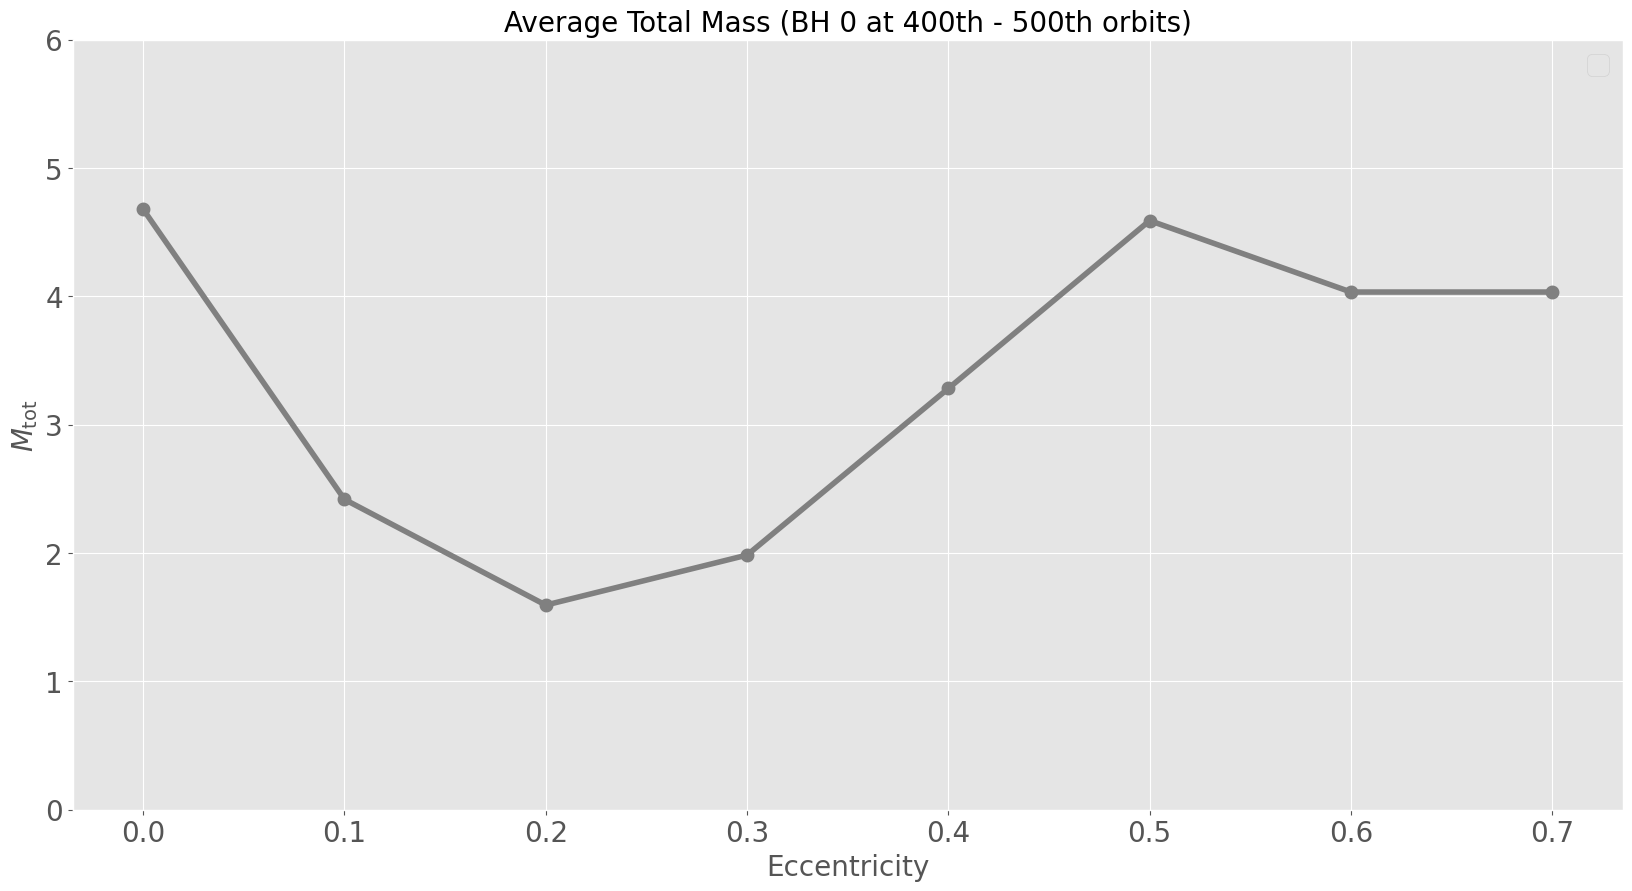
\includegraphics[width=6cm]{minidisk.png}
    \centering
    \end{figure}


\section{Future Work}
We also attempted to look at the trend of the total mass of each minidisk as a function of eccentricity, and we found that there is some periodicity of the mass oscillation
per about 100 orbits. We used Fourier transform to for the biggest period for each eccentricity, but we did not see any consistency among all eccentricities. Below, the plot
shows somewhere around 0.5 frequency, there is overlap, but it can also be caused by the natural rotation of the cavity. 

\begin{figure}[h]
    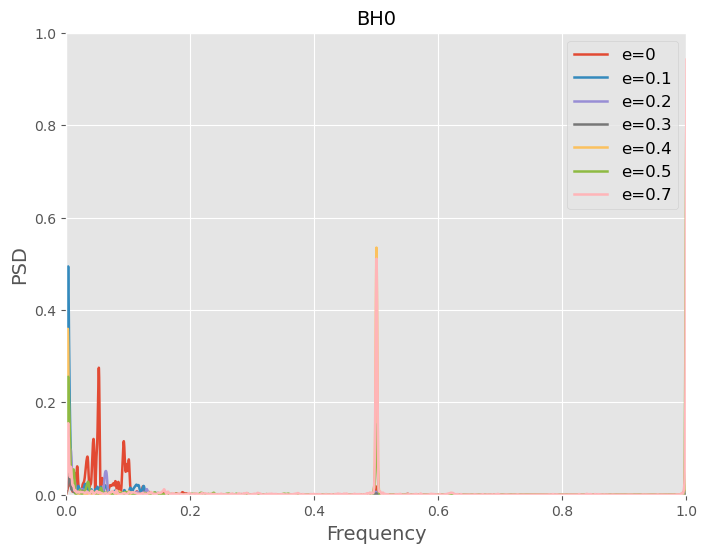
\includegraphics[width=6cm]{frequency.png}
    \centering
    \end{figure}

Some other directions of future works are:

\begin{enumerate}
    \item Investigating if unequal masses of the binary black holes will affect the stable eccentricity point.
    \item Does the total mass of the minidisks depends on other factor such as viscosity or adiabatic index?
    \item Investigating the effects of the total time of the simulation on the total mass of the minidisks.
    \item What other cooling machanisms can we use to cool the disk instead of setting it to isothermal?
\end{enumerate}

\end{document}
